In this chapter we present the different tests that were performed to compare the capabilities of the old and new methods. For each test, the results of both methods of discretization are compared.

In total, four kinds of tests were conducted:
\begin{itemize}
	\item Invariance
	\item Image reconstruction
	\item Image recognition
	\item Template matching
\end{itemize}

\section{Test images}\label{sec:test_images}
The images for testing were acquired from multiple online image libraries. The Lenna and Pepper images~\cite{usc_sipi} (shown on Figure~\ref{fig:lena_pepper_original}) were used to test image reconstruction as well as to demonstrate the different points systems.

\begin{figure}[tbp]
    \begin{subfigure}{0.49\textwidth}
        \centering
    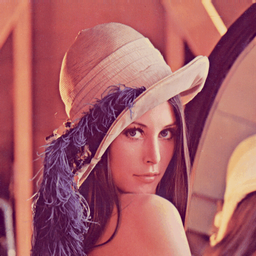
\includegraphics[width=128pt]{figures/lenna_color_256.png}
    \caption{}
	\end{subfigure}
	\begin{subfigure}{0.49\textwidth}
        \centering
    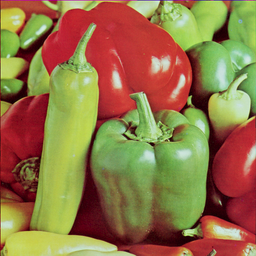
\includegraphics[width=128pt]{figures/pepper_color_256.png}
    \caption{}
	\end{subfigure}
	\caption{The Lenna and Pepper images}
	\label{fig:lena_pepper_original}
\end{figure}

For the image recognition tests, two sets of images were used. The first set consists of 14 images chosen from the Columbia Object Image Library (COIL-100)~\cite{coil}, shown on Figure~\ref{fig:coil_original}. These images are originally $128 \times 128$ pixels, but they were placed on a $204 \times 204$ black background so that the rotated, scaled and translated versions of the images stay completely within these dimensions. 

A set of 1008 rotated images was created by rotating each of the 14 images by a degree $\alpha\in\{0,5,10,\ldots,350,355\}$. Some examples of the extended and rotated images are shown on Figure~\ref{fig:coil_rot}.

Another set of 1176 rotated, scaled and translated images was created by translating each image by -11 pixels in the $x$ direction and 9 pixels in the $y$ direction. Then the translated images were rotated by $\alpha \in \{0,30,60,\ldots,300,330\}$. Finally, each rotated and translated image was scaled by $\lambda \in \{0.5, 0.75, \ldots, 1.75, 2\}$. When either scaling or rotation required, bilinear interpolation was used.
Some examples of the RST transformed images are shown on Figure~\ref{fig:coil_rst}.

\begin{figure}[tbp]
    \begin{subfigure}{80pt}
        \centering
    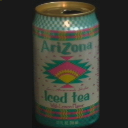
\includegraphics[width=\textwidth]{figures/coil_original/7.png}
    \caption{}
	\end{subfigure}
	\begin{subfigure}{80pt}
        \centering
    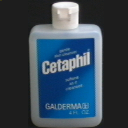
\includegraphics[width=\textwidth]{figures/coil_original/13.png}
    \caption{}
	\end{subfigure}
	\begin{subfigure}{80pt}
        \centering
    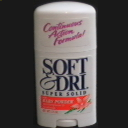
\includegraphics[width=\textwidth]{figures/coil_original/22.png}
    \caption{}
	\end{subfigure}
	\begin{subfigure}{80pt}
        \centering
    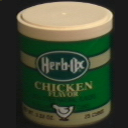
\includegraphics[width=\textwidth]{figures/coil_original/26.png}
    \caption{}
	\end{subfigure}
	\begin{subfigure}{80pt}
        \centering
    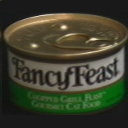
\includegraphics[width=\textwidth]{figures/coil_original/29.png}
    \caption{}
	\end{subfigure}
	\begin{subfigure}{80pt}
        \centering
    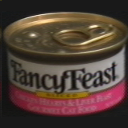
\includegraphics[width=\textwidth]{figures/coil_original/32.png}
    \caption{}
	\end{subfigure}
	\begin{subfigure}{80pt}
        \centering
    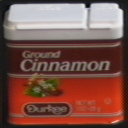
\includegraphics[width=\textwidth]{figures/coil_original/39.png}
    \caption{}
	\end{subfigure}
	\begin{subfigure}{80pt}
        \centering
    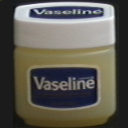
\includegraphics[width=\textwidth]{figures/coil_original/55.png}
    \caption{}
	\end{subfigure}
	\begin{subfigure}{80pt}
        \centering
    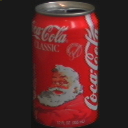
\includegraphics[width=\textwidth]{figures/coil_original/62.png}
    \caption{}
	\end{subfigure}
	\begin{subfigure}{80pt}
        \centering
    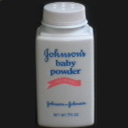
\includegraphics[width=\textwidth]{figures/coil_original/64.png}
    \caption{}
	\end{subfigure}
	\begin{subfigure}{80pt}
        \centering
    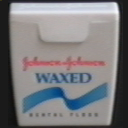
\includegraphics[width=\textwidth]{figures/coil_original/65.png}
    \caption{}
	\end{subfigure}
	\begin{subfigure}{80pt}
        \centering
    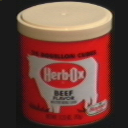
\includegraphics[width=\textwidth]{figures/coil_original/71.png}
    \caption{}
	\end{subfigure}
	\begin{subfigure}{80pt}
        \centering
    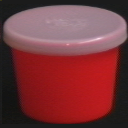
\includegraphics[width=\textwidth]{figures/coil_original/95.png}
    \caption{}
	\end{subfigure}
	\begin{subfigure}{80pt}
        \centering
    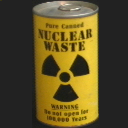
\includegraphics[width=\textwidth]{figures/coil_original/99.png}
    \caption{}
    \end{subfigure}
	\caption{The 14 selected images from the Columbia Object Image Library (COIL-100)}
	\label{fig:coil_original}
\end{figure}

\begin{figure}[tbp]
	\begin{subfigure}{0.30\textwidth}
        \centering
    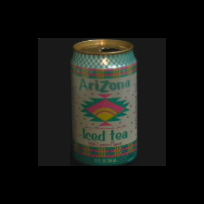
\includegraphics[width=102pt]{figures/coil_rot/7r0.png}
    \caption{$\alpha=0^{\circ}$}
	\end{subfigure}
	\begin{subfigure}{0.30\textwidth}
        \centering
    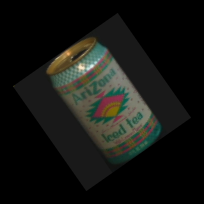
\includegraphics[width=102pt]{figures/coil_rot/7r35.png}
    \caption{$\alpha=35^{\circ}$}
	\end{subfigure}
	\begin{subfigure}{0.30\textwidth}
        \centering
    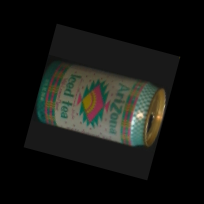
\includegraphics[width=102pt]{figures/coil_rot/7r255.png}
    \caption{$\alpha=255^{\circ}$}
	\end{subfigure}
	\caption{Some extended and rotated images from COIL}
	\label{fig:coil_rot}
\end{figure}

\begin{figure}[tbp]
	\begin{subfigure}{0.29\textwidth}
        \centering
    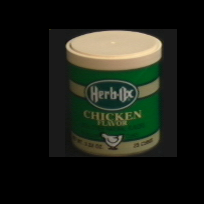
\includegraphics[width=102pt]{figures/coil_rst/26x-11y9r0s1_0.png}
    \caption{$\alpha=0^{\circ}$, $\lambda=1$}
	\end{subfigure}
	\begin{subfigure}{0.28\textwidth}
        \centering
    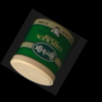
\includegraphics[width=51pt]{figures/coil_rst/26x-11y9r150s0_5.png}
    \caption{$\alpha=150^{\circ}$, $\lambda=0.5$}
	\end{subfigure}
	\begin{subfigure}{0.40\textwidth}
        \centering
    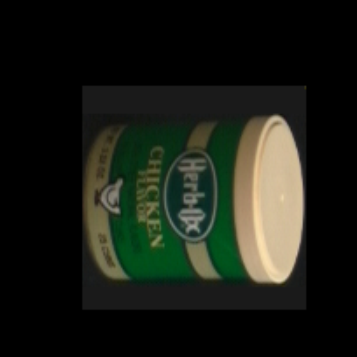
\includegraphics[width=153pt]{figures/coil_rst/26x-11y9r270s1_75.png}
    \caption{$\alpha=270^{\circ}$, $\lambda=1.5$}
	\end{subfigure}
	\caption{Some RST transformed images from COIL. All images are translated by $\Delta x = -11$, $\Delta y = 9$}
	\label{fig:coil_rst}
\end{figure}

Another set of 13 images was acquired from the Amsterdam Library of Object Images (ALOI)~\cite{aloi}. These are shown on Figure~\ref{fig:aloi_original}. Originally, these size of these images was $768 \times 576$ pixels, but the were downscaled to $96 \times 72$ and subsequently extended to $152 \times 128$ by placing the images on a black background. Similarly to the test sets created using the COIL-100 images, the ALOI images were also translated, rotated and scaled, yielding a set of 1092 RST transformed images. The parameters of the transformation were the same as for the COIL-100 images, except for the translation, where $\Delta x = 8$ and $\Delta y = 5$ was used.

\begin{figure}[tbp]
    \begin{subfigure}{80pt}
        \centering
    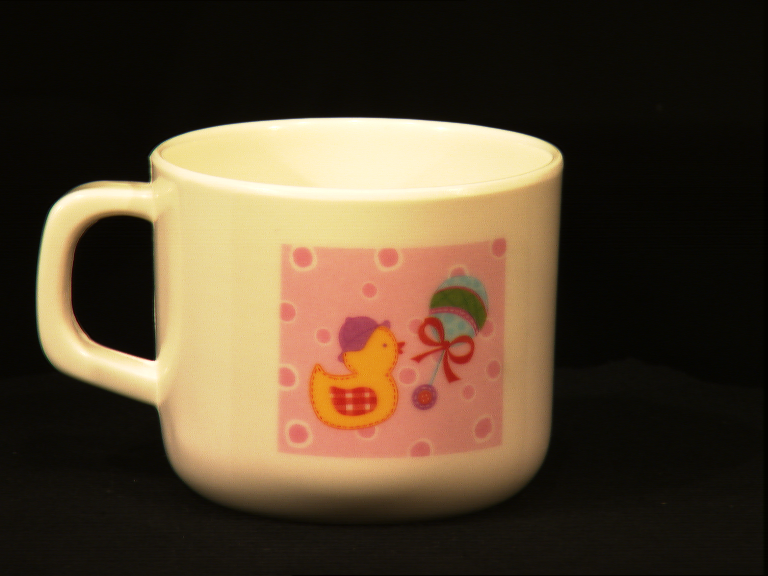
\includegraphics[width=\textwidth]{figures/aloi_original/36.png}
    \caption{}
	\end{subfigure}
	\begin{subfigure}{80pt}
        \centering
    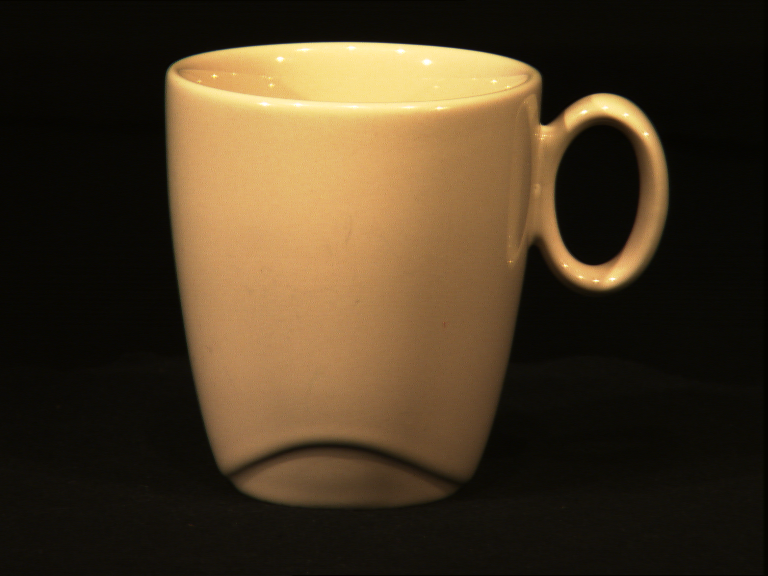
\includegraphics[width=\textwidth]{figures/aloi_original/125.png}
    \caption{}
	\end{subfigure}
	\begin{subfigure}{80pt}
        \centering
    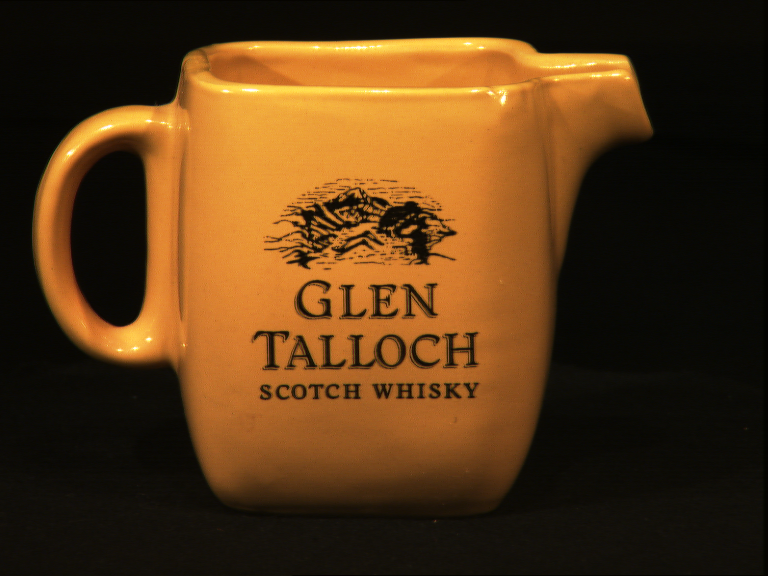
\includegraphics[width=\textwidth]{figures/aloi_original/127.png}
    \caption{}
	\end{subfigure}
	\begin{subfigure}{80pt}
        \centering
    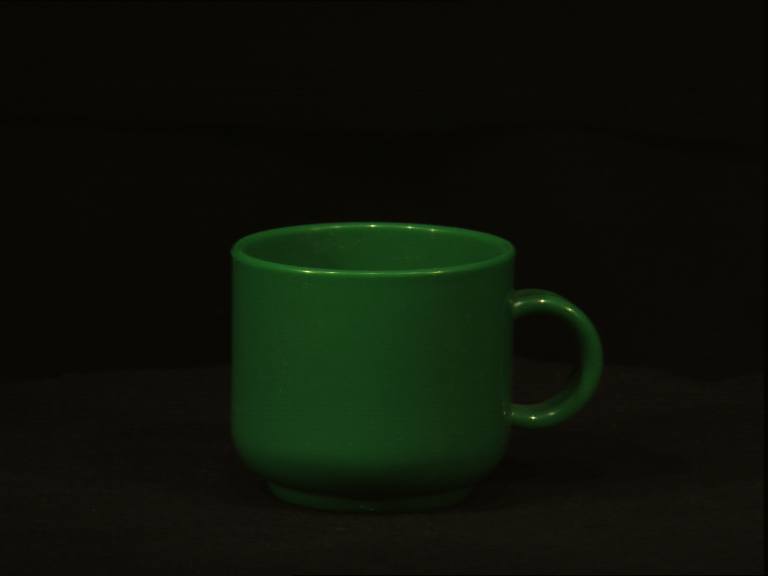
\includegraphics[width=\textwidth]{figures/aloi_original/153.png}
    \caption{}
	\end{subfigure}
	\begin{subfigure}{80pt}
        \centering
    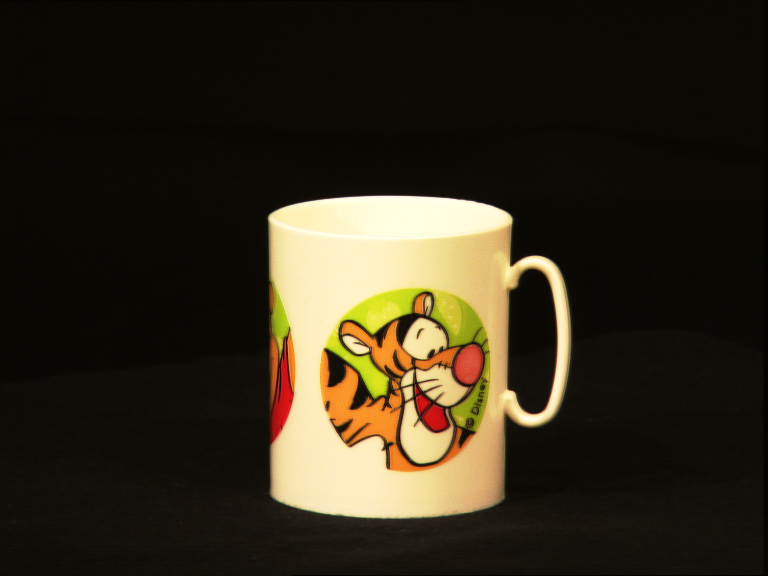
\includegraphics[width=\textwidth]{figures/aloi_original/157.png}
    \caption{}
	\end{subfigure}
	\begin{subfigure}{80pt}
        \centering
    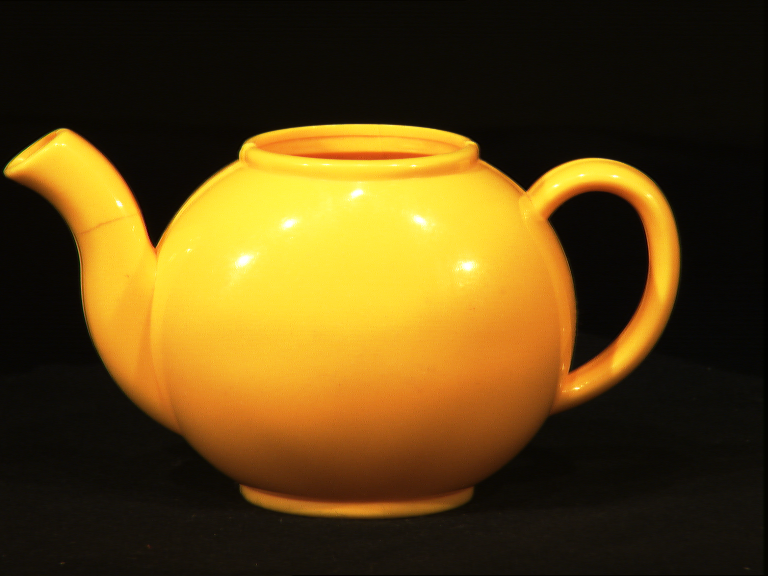
\includegraphics[width=\textwidth]{figures/aloi_original/161.png}
    \caption{}
	\end{subfigure}
	\begin{subfigure}{80pt}
        \centering
    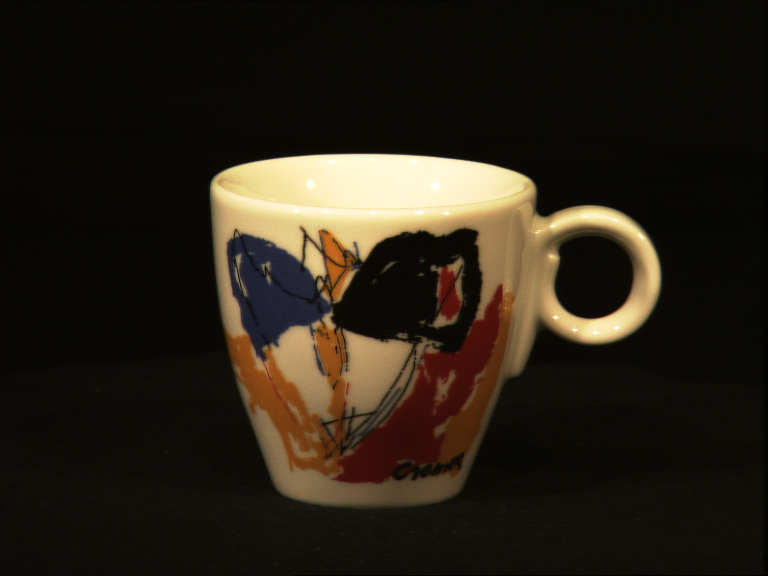
\includegraphics[width=\textwidth]{figures/aloi_original/259.png}
    \caption{}
	\end{subfigure}
	\begin{subfigure}{80pt}
        \centering
    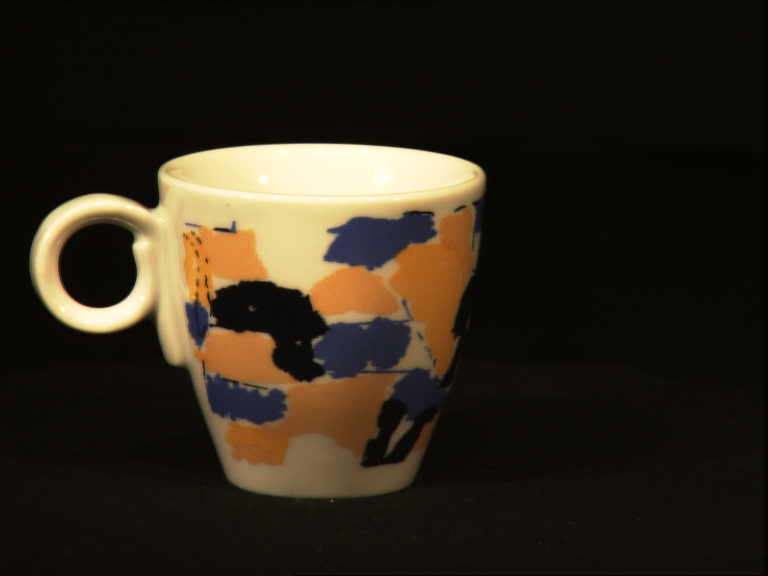
\includegraphics[width=\textwidth]{figures/aloi_original/262.png}
    \caption{}
	\end{subfigure}
	\begin{subfigure}{80pt}
        \centering
    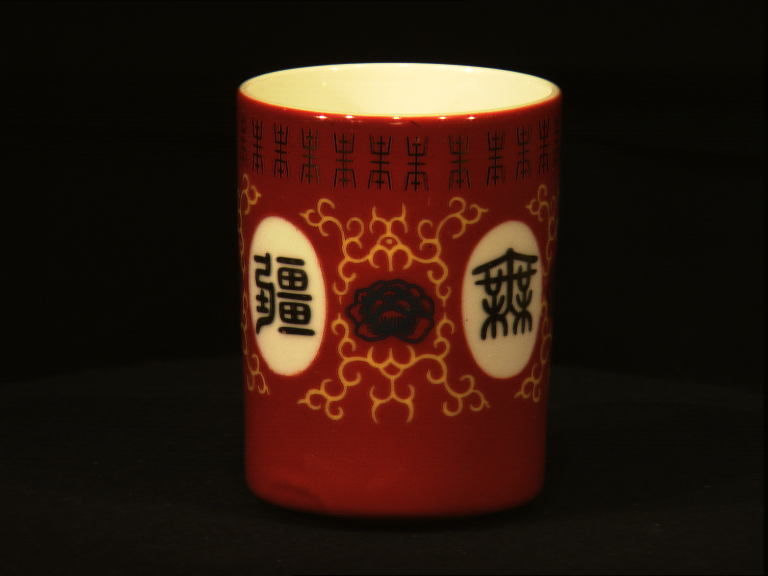
\includegraphics[width=\textwidth]{figures/aloi_original/308.png}
    \caption{}
	\end{subfigure}
	\begin{subfigure}{80pt}
        \centering
    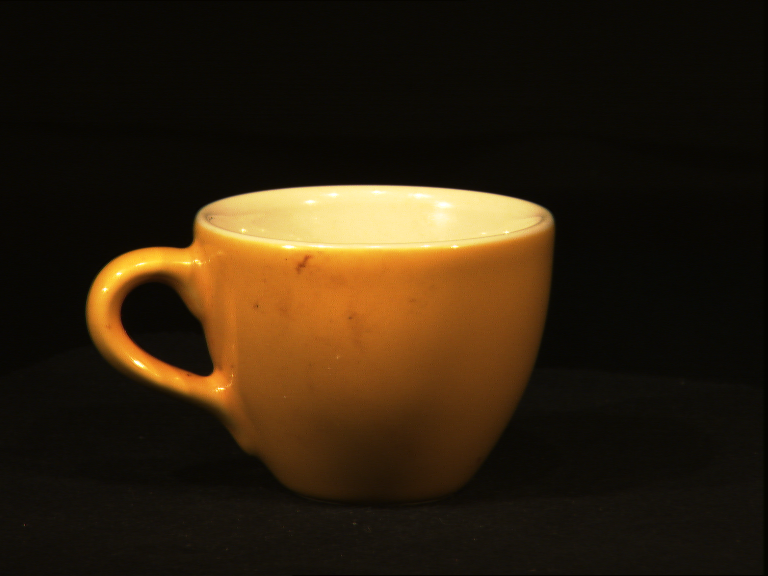
\includegraphics[width=\textwidth]{figures/aloi_original/507.png}
    \caption{}
	\end{subfigure}
	\begin{subfigure}{80pt}
        \centering
    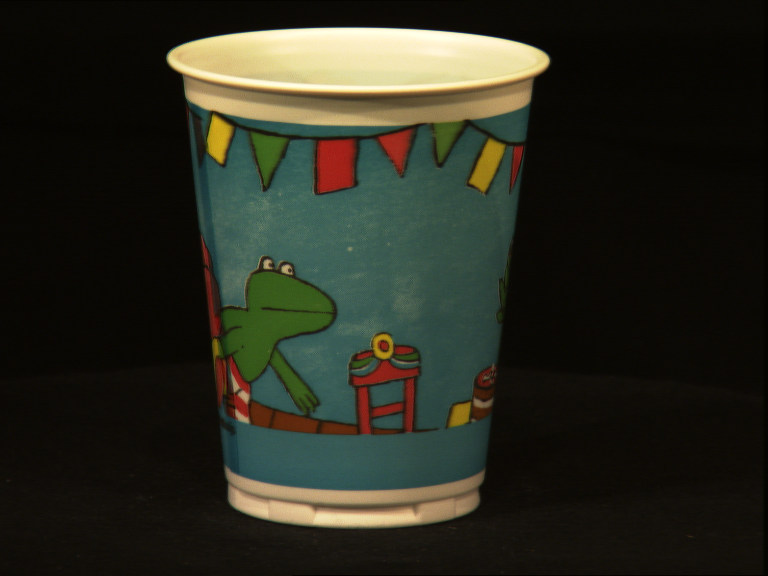
\includegraphics[width=\textwidth]{figures/aloi_original/514.png}
    \caption{}
	\end{subfigure}
	\begin{subfigure}{80pt}
        \centering
    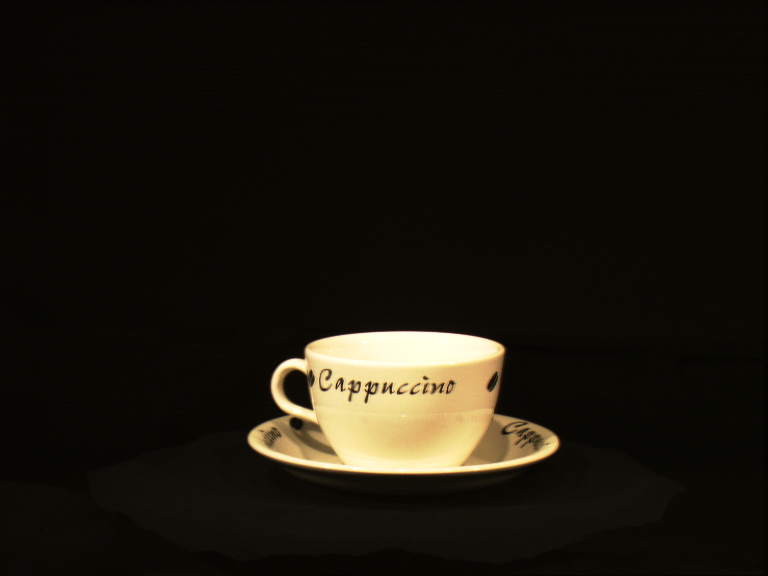
\includegraphics[width=\textwidth]{figures/aloi_original/774.png}
    \caption{}
	\end{subfigure}
	\begin{subfigure}{80pt}
        \centering
    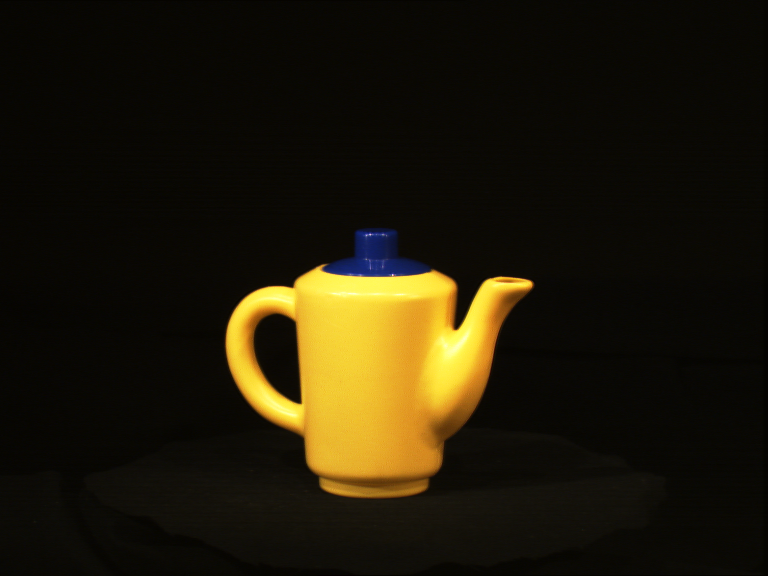
\includegraphics[width=\textwidth]{figures/aloi_original/875.png}
    \caption{}
	\end{subfigure}
	\caption{The 13 selected images from the Amsterdam Library of Object Images (ALOI)}
	\label{fig:aloi_original}

\end{figure}

\section{Invariance test}
In order to test quaternion Zernike moment invariants with respect to rotation, scaling and translation, the QZMIs of order 1 to 4 were calculated for a given image and all of its RST transformations. Then, the modulus of these QZMIs was calculated, as well as the mean ($\mu$), standard deviation ($\sigma$) and $\frac{\sigma}{\mu}$ for the same moment of all transformed images.

\begin{figure}[tbp]
	\begin{subfigure}{0.4\textwidth}
        \centering
    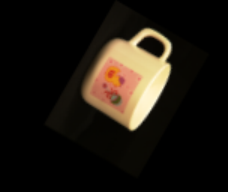
\includegraphics[width=150pt]{figures/inv_img/36x8y5r240s1_5.png}
	\caption{}\label{fig:inv_img1}
	\end{subfigure}
	\begin{subfigure}{0.29\textwidth}
        \centering
    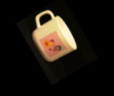
\includegraphics[width=75pt]{figures/inv_img/36x8y5r300s0_75.png}
    \caption{}\label{fig:inv_img2}
	\end{subfigure}
	\begin{subfigure}{0.29\textwidth}
        \centering
    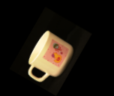
\includegraphics[width=75pt]{figures/inv_img/36x8y5r60s0_75.png}
    \caption{}\label{fig:inv_img3}
	\end{subfigure}
	\begin{subfigure}{0.3\textwidth}
        \centering
    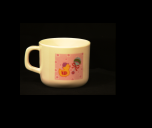
\includegraphics[width=100pt]{figures/inv_img/36x8y5r0s1_0.png}
    \caption{}\label{fig:inv_img4}
	\end{subfigure}
	\begin{subfigure}{0.3\textwidth}
        \centering
    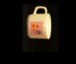
\includegraphics[width=50pt]{figures/inv_img/36x8y5r270s0_5.png}
    \caption{}\label{fig:inv_img5}
	\end{subfigure}
	\begin{subfigure}{0.3\textwidth}
        \centering
    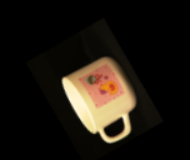
\includegraphics[width=125pt]{figures/inv_img/36x8y5r120s1_25.png}
    \caption{}\label{fig:inv_img6}
	\end{subfigure}
	\caption{The images with different rotation and scale, which are used to test the invariance of the methods.}
	\label{fig:inv_img}
\end{figure}

\subsection{Results}
The moduli of the QZMIs for the transformed images shown on Figure~\ref{fig:inv_img} is shown in Table~\ref{tab:inv_old} for the old method of discretization and in Table~\ref{tab:inv_new} for the new, proposed method of discretization. The coefficient of variation ($\frac{\sigma}{\mu}$) shows that using both methods, the moments are invariant to RST transformation. The only rows where $\frac{\sigma}{\mu}$ is higher are the ones where the modulus of the moment is very close to zero, and thus small numerical errors impact this number significantly. Comparing the two methods, the proposed one yields slightly lower values for the coefficient of variation for all moments.

\begin{table}
	\centering
\begin{tabular}{| c || c | c | c | c | c | c || c | } \hline
& Fig.\ref{fig:inv_img1} & Fig.\ref{fig:inv_img2} & Fig.\ref{fig:inv_img3} & Fig.\ref{fig:inv_img4} & Fig.\ref{fig:inv_img5} & Fig.\ref{fig:inv_img6} & $\frac{\sigma}{\mu}$ \\ \hline\hline
$|\overline{\Psi}_{1,1}^1|$ & 1.50e-2 & 1.58e-2 & 1.54e-2 & 1.61e-2 & 1.58e-2 & 1.49e-2 & 3.73\% \\ \hline
$|\overline{\Psi}_{2,0}^0|$ & 2.965 & 2.964 & 2.964 & 2.963 & 2.964 & 2.965 & 0.028\% \\ \hline
$|\overline{\Psi}_{2,2}^0|$ & 8.793 & 8.785 & 8.789 & 8.783 & 8.786 & 8.794 & 0.057\% \\ \hline
$|\overline{\Psi}_{2,2}^2|$ & 1.50e-4 & 1.65e-4 & 1.57e-4 & 1.69e-4 & 1.65e-4 & 1.47e-4 & 6.87\% \\ \hline
$|\overline{\Psi}_{3,1}^1|$ & 5.91e-2 & 6.25e-2 & 6.09e-2 & 6.34e-2 & 6.22e-2 & 5.89e-2 & 3.71\%  \\ \hline
$|\overline{\Psi}_{3,3}^1|$ & 0.233 & 0.247 & 0.241 & 0.250 & 0.246 & 0.233 & 3.69\% \\ \hline
$|\overline{\Psi}_{3,3}^3|$ & 1.43e-6 & 1.61e-6 & 1.50e-6 & 1.67e-6 & 1.62e-6 & 1.38e-6 & 9.40\% \\ \hline
$|\overline{\Psi}_{4,0}^0|$ & 4.827 & 4.821 & 4.824 & 4.820 & 4.822 & 4.828 & 0.086\% \\ \hline
$|\overline{\Psi}_{4,2}^0|$ & 14.316 & 14.291 & 14.302 & 14.284 & 14.292 & 14.318 & 0.114\% \\ \hline
$|\overline{\Psi}_{4,2}^2|$ & 7.39e-4 & 8.13e-4 & 7.74e-4 & 8.35e-4 & 8.12e-4 & 7.26e-4 & 6.85\% \\ \hline
$|\overline{\Psi}_{4,4}^0|$ & 23.309 & 23.249 & 23.276 & 23.232 & 23.251 & 23.314 & 0.171\% \\ \hline
$|\overline{\Psi}_{4,4}^2|$ & 3.64e-3 & 4.00e-3 & 3.81e-3 & 4.11e-3 & 4.00e-3 & 3.58e-3 & 6.83\% \\ \hline
$|\overline{\Psi}_{4,4}^4|$ & 1.28e-8 & 1.52e-8 & 1.39e-8 & 1.59e-8 & 1.51e-8 & 1.25e-8 & 12.00\% \\ \hline
\end{tabular}
\caption{The modulus of QZMIs using the old method for discretization. Note that $\frac{\sigma}{\mu}$ was calculated using the QZMIs for all transformation of the image, not juts the values shown in the table.}
\label{tab:inv_old}
\end{table}

\begin{table}
	\centering
\begin{tabular}{| c || c | c | c | c | c | c || c | } \hline
& Fig.\ref{fig:inv_img1} & Fig.\ref{fig:inv_img2} & Fig.\ref{fig:inv_img3} & Fig.\ref{fig:inv_img4} & Fig.\ref{fig:inv_img5} & Fig.\ref{fig:inv_img6} & $\frac{\sigma}{\mu}$ \\ \hline\hline
$|\overline{\Psi}_{1,1}^1|$ & 1.49e-2 & 1.58e-2 & 1.54e-2 & 1.60e-2 & 1.57e-2 & 1.49e-2 & 3.72\% \\ \hline
$|\overline{\Psi}_{2,0}^0|$ & 2.965 & 2.964 & 2.964 & 2.963 & 2.964 & 2.965 & 0.028\%\\ \hline
$|\overline{\Psi}_{2,2}^0|$ & 8.793 & 8.785 & 8.789 & 8.783 & 8.786 & 8.793 & 0.056\%\\ \hline
$|\overline{\Psi}_{2,2}^2|$ & 1.49e-4 & 1.64e-4 & 1.55e-4 & 1.68e-4 & 1.63e-4 & 1.47e-4 & 6.82\%\\ \hline
$|\overline{\Psi}_{3,1}^1|$ & 5.90e-2 & 6.25e-2 & 6.08e-2 & 6.33e-2 & 6.21e-2 & 5.89e-2 & 3.70\%\\ \hline
$|\overline{\Psi}_{3,3}^1|$ & 0.233 & 0.247 & 0.240 & 0.250 & 0.245 & 0.233 & 3.68\%\\ \hline
$|\overline{\Psi}_{3,3}^3|$ & 1.41e-6 & 1.61e-6 & 1.48e-6 & 1.65e-6 & 1.60e-6 & 1.37e-6 & 9.32\%\\ \hline
$|\overline{\Psi}_{4,0}^0|$ & 4.828 & 4.821 & 4.824 & 4.820 & 4.822 & 4.828 & 0.085\%\\ \hline
$|\overline{\Psi}_{4,2}^0|$ & 14.317 & 14.291 & 14.304 & 14.286 & 14.293 & 14.318 & 0.113\%\\ \hline
$|\overline{\Psi}_{4,2}^2|$ & 7.35e-4 & 8.13e-4 & 7.68e-4 & 8.29e-4 & 8.07e-4 & 7.25e-4 & 6.80\%\\ \hline
$|\overline{\Psi}_{4,4}^0|$ & 23.312 & 23.249 & 23.279 & 23.236 & 23.254 & 23.314 & 0.170\%\\ \hline
$|\overline{\Psi}_{4,4}^2|$ & 3.62e-3 & 4.00e-3 & 3.79e-3 & 4.09e-3 & 3.98e-3 & 3.58e-3 & 6.78\%\\ \hline
$|\overline{\Psi}_{4,4}^4|$ & 1.28e-8 & 1.52e-8 & 1.37e-8 & 1.56e-8 & 1.50e-8 & 1.24e-8 & 11.94\%\\ \hline
\end{tabular}
\caption{The modulus of QZMIs using the new method for discretization. Note that $\frac{\sigma}{\mu}$ was calculated using the QZMIs for all transformation of the image, not juts the values shown in the table.}
\label{tab:inv_new}
\end{table}

\section{Image reconstruction}
As described in Section~\ref{sec:qzm}, the quaternion Zernike moments of an image can be used to approximately reconstruct the original image using the formulas in \eqref{eq:qzm_reconstruction}. This reconstruction requires the computation of QZMs of up to a finite degree $M$.

In order to reconstruct the discrete image, formula 
$$
f(r_{x,y},\theta_{x,y}) \approx \sum_{n=0}^{M}\sum_{m=-n}^{n}Z_{n,m}^R(f)R_{n,m}(r_{x,y})e^{\bm{\mu}m\theta_{x,y}}
$$
was used for each pixel with image coordinates $(x,y)$, where $(r_{x,y},\theta_{x,y})$ are the polar coordinates obtained by performing the linear transformation of the image onto the unit disk, using the transformation shown on Figure~\ref{fig:transform1} (\textit{tf\textsubscript{1}}) for the old method and the transformation shown on Figure~\ref{fig:transform2} (\textit{tf\textsubscript{2}}) for the new one. The reason for this difference in transformation is that for the proposed discrete orthogonal points system, the interpolated pixel values are calculated using \textit{tf\textsubscript{2}}, while conventionally for (quaternion) Zernike moments, \textit{tf\textsubscript{1}} is used~\cite{qzmi}.

To measure the error of the reconstruction the normalized mean squared error ($\varepsilon^2$) was used. If $f(x,y)$ is the original and $\widehat{f}(x,y)$ is the reconstructed image, both with size $N \times N$, then the normalized mean squared error is defined as:
\begin{gather*}
    \varepsilon^2 = \frac{\displaystyle \sum_{x=1}^N\sum_{y=1}^N \left|f(x,y) - \widehat{f}(x,y)\right|^2}{\displaystyle \sum_{x=1}^N\sum_{y=1}^N \left|f(x,y)\right|^2}.
\end{gather*}

In the cases, where \textit{tf\textsubscript{2}} is used only the part of the image falling inside the unit circle is reconstructed and thus the mean squared error is calculated over only this part of the image.

For the new method of discretization the number of points on the unit disk was chosen to be approximately the same as the number of pixels falling inside the inscribed circle of the image. 

\subsection{Results}
Image reconstruction was performed for both the Lenna and the Pepper images~\cite{usc_sipi}, using image sizes ranging from $64\times 64$ up to $256 \times 256$. Depending on the size of the image, QZMs of up to degree 350 were used reconstruct the image. However, in the case of smaller images, for example a $64\times 64$ image, only QZMs of up to 100 degree could be used, as using higher degrees would result in trying to extract more information from the original image than there is information contained in the pixel values, thus increasing the error of reconstruction. This phenomenon is visible, for example on Figure~\ref{fig:reconstruction_new} for the $64 \times 64$ Lenna, M = 100 case.

Figure~\ref{fig:reconstruction_old} shows some of the reconstructed images and their normalized mean squared error when using the old method of discretization, while Figure~\ref{fig:reconstruction_new} shows the same data using the new method.

Comparing the error of reconstruction between the two methods, using the discrete orthogonal points system provides much lower normalized mean squared errors for almost all levels of reconstruction. 
Table~\ref{tab:epsilons} shows the comparison between the $\varepsilon^2$ values and the change in the error when using the proposed method instead of the old one. The decrease in the error of reconstruction is is significant for both low and high maximal degrees of QZMs. 

Due to the lower number of points used by the second method (because of the different transformation of the image onto the unit disk) the previously described increase in reconstruction error occurs for lower $M$s than in the original method.

\newcolumntype{Q}{>{\centering\arraybackslash} m{64pt} }
\newcolumntype{q}{>{\centering\arraybackslash} m{50pt} }

\begin{figure}
	\centering
\begin{tabular}{q | Q Q Q Q }
M & Lenna $64\times 64$& Lenna $128\times 128$ & Lenna $256 \times 256$ & Pepper $256 \times 256$\\ \hline\hline
Original & 

\includegraphics[width=64pt]{figures/reconstruction/lo64.png} & 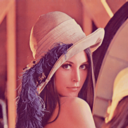
\includegraphics[width=64pt]{figures/reconstruction/lo128.png} & 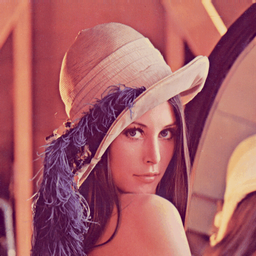
\includegraphics[width=64pt]{figures/reconstruction/lo256.png} & 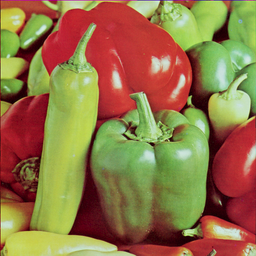
\includegraphics[width=64pt]{figures/reconstruction/po256.png}\\\hline
M = 50 & 
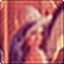
\includegraphics[width=64pt]{figures/reconstruction/lo6450.png} & 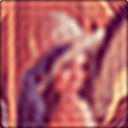
\includegraphics[width=64pt]{figures/reconstruction/lo12850.png} & 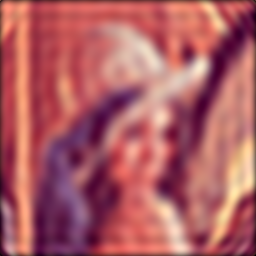
\includegraphics[width=64pt]{figures/reconstruction/lo25650.png} & 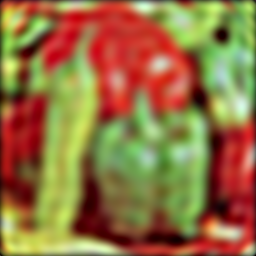
\includegraphics[width=64pt]{figures/reconstruction/po25650.png}\\
& 0.01257 & 0.01948 & 0.02659 & 0.03777\\
M = 100 & 

\includegraphics[width=64pt]{figures/reconstruction/lo64100.png} & \includegraphics[width=64pt]{figures/reconstruction/lo128100.png} & \includegraphics[width=64pt]{figures/reconstruction/lo256100.png} & \includegraphics[width=64pt]{figures/reconstruction/po256100.png}\\
& 0.00468 & 0.00719 & 0.01341 & 0.01596\\
M = 150 & & 
\includegraphics[width=64pt]{figures/reconstruction/lo128150.png} & \includegraphics[width=64pt]{figures/reconstruction/lo256150.png} & \includegraphics[width=64pt]{figures/reconstruction/po256150.png}\\
& & 0.00388 & 0.00868 & 0.00885\\
M = 250 & & & 
\includegraphics[width=64pt]{figures/reconstruction/lo256250.png} & \includegraphics[width=64pt]{figures/reconstruction/po256250.png}\\
& & & 0.00428 & 0.00378\\
M = 350 & & & 
\includegraphics[width=64pt]{figures/reconstruction/lo256350.png} & \includegraphics[width=64pt]{figures/reconstruction/po256350.png}\\
& & & 0.00279 & 0.00253\\
& \\

\end{tabular}
\caption{Reconstructed images using the old method, with the normalized mean squared error shown below each image.}
\label{fig:reconstruction_old}
\end{figure}

\begin{figure}
	\centering
\begin{tabular}{q | Q Q Q Q }
M & Lenna $64\times 64$& Lenna $128\times 128$ & Lenna $256 \times 256$ & Pepper $256 \times 256$\\ \hline\hline
Original & 
\includegraphics[width=64pt]{figures/reconstruction/lo64.png} & \includegraphics[width=64pt]{figures/reconstruction/lo128.png} & \includegraphics[width=64pt]{figures/reconstruction/lo256.png} & \includegraphics[width=64pt]{figures/reconstruction/po256.png}\\\hline
M = 50 &
\includegraphics[width=64pt]{figures/reconstruction/ln6450.png} & \includegraphics[width=64pt]{figures/reconstruction/ln12850.png} & \includegraphics[width=64pt]{figures/reconstruction/ln25650.png} & \includegraphics[width=64pt]{figures/reconstruction/pn25650.png}\\
& 0.00380 & 0.00901 & 0.01611 & 0.01778\\
M = 100 & 
\includegraphics[width=64pt]{figures/reconstruction/ln64100.png} & \includegraphics[width=64pt]{figures/reconstruction/ln128100.png} & \includegraphics[width=64pt]{figures/reconstruction/ln256100.png} & \includegraphics[width=64pt]{figures/reconstruction/pn256100.png}\\
& 0.01181 & 0.00246 & 0.00790 & 0.00681\\
M = 150 & & 
\includegraphics[width=64pt]{figures/reconstruction/ln128150.png} & \includegraphics[width=64pt]{figures/reconstruction/ln256150.png} & \includegraphics[width=64pt]{figures/reconstruction/pn256150.png}\\
& & 0.00152 & 0.00463 & 0.00349\\
M = 250 & & & 
\includegraphics[width=64pt]{figures/reconstruction/ln256250.png} & \includegraphics[width=64pt]{figures/reconstruction/pn256250.png}\\
& & & 0.00190 & 0.00131\\
M = 350 & & & 
\includegraphics[width=64pt]{figures/reconstruction/ln256350.png} & \includegraphics[width=64pt]{figures/reconstruction/pn256350.png}\\
& & & 0.00238 & 0.00229\\
& \\

\end{tabular}
\caption{Reconstructed images using the proposed new method, with the normalized mean squared error shown below each image.}
\label{fig:reconstruction_new}
\end{figure}

\begin{table}
    \centering
    \begin{tabular}{|c||c|c|c|c|c|}
        M & 50 & 100 & 150 & 250 & 350 \\ \hline
        old method $\varepsilon^2$ & 0.02659 & 0.01341 & 0.00868 & 0.00428 & 0.00279 \\ 
        new method $\varepsilon^2$ & 0.01611 & 0.00790 & 0.00463 & 0.00190 & 0.00238 \\ \hline
        change & -39.4\% & -41.1\% & -46.7\% & -55.6\% & -14.7\% \\
    \end{tabular}
    \caption{Comparison of the normalized mean squared errors between the two method, for the $256 \times 256$ Lenna image.}
    \label{tab:epsilons}
\end{table}

\section{Image recognition}
In order to test image recognition capabilities, the COIL-100~\cite{coil} and ALOI~\cite{aloi} images and the RST transformed sets of images were used. The exact parameters for the transformations performed to obtain these sets of images is described in Section~\ref{sec:test_images}.
The goal of the image recognition test is to see what percentage of the transformed images can each method correctly identify by comparing their moment invariants to the ones of the original, non-transformed images.

To recognize an image, first the QZMIs have to be calculated. In this thesis, we used QZMIs of up to degree 4, but not all possible QZMIs were used. The selected QZMIs were: $\overline{\Psi}_{1,1}^1, \overline{\Psi}_{2,0}^0, \overline{\Psi}_{2,2}^2, \overline{\Psi}_{3,1}^1, \overline{\Psi}_{3,3}^3, \overline{\Psi}_{4,0}^0, \overline{\Psi}_{4,2}^2, \overline{\Psi}_{4,4}^4$. These 8 quaternion valued invariants contain a total of 20 real valued invariants, since while each quaternion could provide of 4 real invariants, the QZMIs $\overline{\Psi}_{n,k}^m$ with $n = k$ necessarily have $\ip{\overline{\Psi}_{n,n}^m} = 0$.
This follows directly from the definition (see Section~\ref{sec:invariance}): 
\begin{gather*}
    \begin{split}
        \overline{\Psi}_{n,n}^m &= \overline{L}_{n,m}^R(f)(\overline{L}_{n,m}^R(f))^* = \left|\overline{L}_{n,m}^R(f)\right|^2 \in \R.
    \end{split}
\end{gather*}
Thus from the selected 8 QZMIs four provide a single real-valued invariant and another four provide 4 real-valued invariants. These 20 real invariants are then used to construct a vector $I$ of length 20.
This vector is normalized using the method presented by \citeauthor{affine_color}~\cite{affine_color}.
$$
I_k = sgn(I_k)\left|I_k\right|^\frac{1}{2} \;\;\;\; (k = 1,2,\ldots,20).
$$

This invariant vector is calculated for an RST transformed image and all of the original images. Then the minimum Euclidean distance is used to choose from the original images. The recognition algorithm classifies the transformed image as this chosen image.

\subsection{Noise generation}
To test robustness against noise the tests were also performed with different levels of real-valued Gaussian noise added to all images. The parameters of the Gaussian noise were as follows: the mean of the distribution was always at 0, while standard deviation ($\sigma$) values from 1 up to 60 were used for the QZMIs and standard deviation ranging from 40 to 120 was used to test the QZMRIs. QZMRIs are more robust against noise than QZMIs, so higher noise values could be used.
Instead of using Gaussian noise, for some test cases salt-and-pepper noise was added with densities ($p$) ranging from 0.2\% up to 15\% for the QZMIs and ranging from 5\% to 30\% for the QZMRIs. Some examples for both types of noise are shown on Figure~\ref{fig:noise}.


The tests were performed directly using the raw, noisy images, without any kind of filtering applied to the image. The goal was to see the robustness of these methods against noise. 

\begin{figure}[tbp]
	\begin{subfigure}{0.329\textwidth}
        \centering
    \includegraphics[width=\textwidth]{figures/noise/gauss3.png}
	\caption{$\sigma = 3$}
	\end{subfigure}
    \begin{subfigure}{0.329\textwidth}
        \centering
    \includegraphics[width=\textwidth]{figures/noise/gauss5.png}
	\caption{$\sigma = 5$}
    \end{subfigure}
    \begin{subfigure}{0.329\textwidth}
        \centering
    \includegraphics[width=\textwidth]{figures/noise/gauss7.png}
	\caption{$\sigma = 7$}
    \end{subfigure}
    \begin{subfigure}{0.329\textwidth}
        \centering
    \includegraphics[width=\textwidth]{figures/noise/pepper04.png}
	\caption{$p = 0.4\%$}
    \end{subfigure}
    \begin{subfigure}{0.329\textwidth}
        \centering
    \includegraphics[width=\textwidth]{figures/noise/pepper1.png}
	\caption{$p = 1\%$}
    \end{subfigure}
    \begin{subfigure}{0.329\textwidth}
        \centering
    \includegraphics[width=\textwidth]{figures/noise/pepper3.png}
	\caption{$p = 3\%$}
	\end{subfigure}
	\caption{Some test images with Gaussian noise (top row) or salt-and-pepper noise (bottom row) with different parameters added to them.}
	\label{fig:noise}
\end{figure}

\subsection{Test cases}
The recognition tests were performed using both the old and the proposed method for discretization. Furthermore, the new method was tested with with two different $N$ values for creating the discrete orthogonal system of $8N^2$ points.

In the first case $N$ was chosen such that the total number of points in the system should be approximately the same as the pixels of the image falling inside its inscribed circle.
\begin{gather*}
    \begin{split}
    N &\in \N \\
    8N^2 &\approx n^2\frac{\pi}{4} \\
    N &= \left\lfloor 2n\sqrt{\pi}\right\rfloor.
    \end{split}
\end{gather*}
where the size of the image is $n \times n$. Based on the interpolating methods described in Section~\ref{sec:new_trans} this means that bilinear interpolation should be used.

In the other case $N$ was chosen such that the number of points is close to the minimum required to achieve discrete orthogonality of moments up to degree 4. In this case $N = 10$ was chosen.
Since the number of points is far less then the number of pixels, based on Section~\ref{sec:new_trans} the interpolation should be done using the integral interpolation formula.

Note that for the old method, the number of points used is the same as the number of pixels in the image.

Three sets of transformed images were tested, which were generated as described in Section~\ref{sec:test_images}:
\begin{itemize}
    \item COIL-100 rotated (1008 images)
    \item COIL-100 rotated, scaled, translated (1176 images)
    \item ALOI rotated, scaled, translated (1092 images)
\end{itemize} 
For the set where only rotation was applied to the images, instead of using QZMIs the rotation invariant QZMRIs were used.

\subsection{Results}

\begin{table}[tbp]
    \centering
    \begin{tabular}{|p{2.15cm}|p{1.8cm}|p{3cm}|p{2.74cm}|p{2.6cm}|} \hline
        \textbf{Image set} & \textbf{Noise stdev.} & \textbf{Old method} (\%) & \textbf{New method} many points (\%)& \textbf{New method} few points (\%) \\ \hline\hline
        COIL - RST & No noise & 99.06 & 99.15 & 98.21 \\ \cline{2-5}
        & 1 & 98.98 & 99.49 & 98.81 \\ \cline{2-5}
        & 2 & 98.98 & 99.74 & 98.81 \\ \cline{2-5}
        & 3 & 98.55 & 99.83 & 98.04 \\ \cline{2-5}
        & 5 & 95.15 & 99.49 & 94.64 \\ \cline{2-5}
        & 7 & 95.15 & 98.72 & 91.67 \\ \cline{2-5}
        & 9 & 76.87 & 98.47 & 89.20 \\ \cline{2-5}
        & 40 & 52.89 & 88.52 & 51.87 \\ \cline{2-5}
        & 50 & 48.21 & 84.10 & 45.07 \\ \cline{2-5}
        & 60 & 41.58 & 85.80 & 39.12 \\ \hline\hline
        ALOI - RST & No noise & 99.91 & 100.00 & 94.60 \\ \cline{2-5}
        & 1 & 94.51 & 99.08 & 86.63 \\ \cline{2-5}
        & 2 & 84.89 & 93.13 & 86.35 \\ \cline{2-5}
        & 3 & 78.85 & 88.55 & 74.81 \\ \cline{2-5}
        & 5 & 72.07 & 93.31 & 58.24 \\ \cline{2-5}
        & 7 & 63.28 & 94.23 & 61.81 \\ \cline{2-5}
        & 9 & 55.04 & 94.32 & 48.81 \\ \cline{2-5}
        & 40 & 18.41 & 90.84 & 15.29 \\ \cline{2-5}
        & 50 & 19.32 & 82.51 & 15.93 \\ \cline{2-5}
        & 60 & 13.19 & 84.89 & 13.83 \\ \cline{1-5}
    \end{tabular}
    \caption{Percentage of images recognized correctly by QZMIs in the case of using the RST transformed image sets with added Gaussian noise.}
    \label{tab:recognition_gauss}
\end{table}
When the images have Gaussian noise, the new method with the higher number of points performs the best for all levels of noise, far outperforming the original method in recognition capabilities. 
The rate of recognition for Gaussian noise in case of the RST transformed image sets is shown in Table~\ref{tab:recognition_gauss}. The recognition rate of the new method remains relatively high (around 80\%) even for high noise values, while the recognition rate of the original method drops significantly (below 20\% in some cases).

When using only the minimal possible number of points in the new method, for all noise levels the recognition rate remains roughly around the same level as with the original method, but the computation required to achieve such levels of image recognition is much lower because of the lower number of points.

The same observation can be made about the QZMRIs used to recognize the rotated images. Even for extremely high noise values, the recognition rate of the new method remains well above 90\%. The results for the QZMRIs are shown in Table~\ref{tab:recognition_rot}.

The reason for such differences between the old and the new methods is that the old method uses a non-orthogonal discretization, which means some redundancy occurs among the QZMs. This leads to the value of the added increasing when these QZMs are multiplied to construct the QZMIs. On the other hand, the new method uses a discrete orthogonal system, which means no redundancy between the QZMs and thus it more robust against Gaussian noise.

When salt-and-pepper noise is added to the images, the recognition capabilities of both methods are high, but no clear difference is visible between them. Even using the minimal possible number of points in the new method, the recognition rates are almost the same as with the other two methods. 
These same observation can be made about the recognition capabilities of the QZMRIs.
The results for salt-and-pepper noise are shown for QZMIs and QZMRIs in Table~\ref{tab:recognition_salt} and Table~\ref{tab:recognition_rot} respectively.

The reason for no significant difference between the methods in the case of salt-and-pepper noise is that this kind of noise adds a high frequency component to the image. Choosing only moments with low order for image recognition behaves as a low-pass filter, since these moments are most sensitive to low frequency components. Thus both methods are able to handle salt-and-pepper noise well.

\begin{table}
    \centering
    \begin{tabular}{|p{2.15cm}|p{1.8cm}|p{3cm}|p{2.74cm}|p{2.6cm}|} \hline
        \textbf{Noise type} & \textbf{Noise param.} & \textbf{Old method} (\%) & \textbf{New method} many points (\%)& \textbf{New method} few points (\%) \\ \hline\hline
        No noise & & 100.00 & 100.00 & 100.00 \\ \hline\hline
        Gauss & 40 & 91.37 & 99.90 & 92.56 \\ \cline{2-5}
        & 50 & 86.51 & 100.00 & 94.44 \\ \cline{2-5}
        & 60 & 84.42 & 99.60 & 93.35 \\ \cline{2-5}
        & 70 & 80.85 & 99.90 & 83.93 \\ \cline{2-5}
        & 80 & 76.98 & 98.12 & 80.45 \\ \cline{2-5}
        & 90 & 75.79 & 99.01 & 83.83 \\ \cline{2-5}
        & 100 & 64.98 & 98.91 & 79.46 \\ \cline{2-5}
        & 110 & 64.78 & 97.62 & 69.94 \\ \cline{2-5}
        & 120 & 68.55 & 96.23 & 72.12 \\ \hline\hline
        Salt & 5 & 100.00 & 100.00 & 100.00 \\ \cline{2-5}
        & 10 & 100.00 & 100.00 & 100.00 \\ \cline{2-5}
        & 15 & 100.00 & 100.00 & 100.00 \\ \cline{2-5}
        & 20 & 100.00 & 100.00 & 100.00 \\ \cline{2-5}
        & 25 & 100.00 & 100.00 & 100.00 \\ \cline{2-5}
        & 30 & 100.00 & 100.00 & 100.00 \\ \cline{1-5}
    \end{tabular}
    \caption{Percentage of images recognized correctly by QZMRIs in the case of using the rotated COIL image set with either Gaussian or salt-and-pepper noise. The noise parameter means the standard deviation in case of the Gaussian noise, and the density in case of the salt-and-pepper noise.}
    \label{tab:recognition_rot}
\end{table}

\begin{table}
    \centering
    \begin{tabular}{|p{2.15cm}|p{1.8cm}|p{3cm}|p{2.74cm}|p{2.6cm}|} \hline
        \textbf{Image set} & \textbf{Noise density} & \textbf{Old method} (\%) & \textbf{New method} many points (\%)& \textbf{New method} few points (\%) \\ \hline\hline
        COIL - RST & No noise & 99.06 & 99.15 & 98.21 \\ \cline{2-5}
        & 0.2 & 99.66 & 99.32 & 94.98 \\ \cline{2-5}
        & 0.4 & 99.91 & 99.74 & 99.15 \\ \cline{2-5}
        & 0.6 & 99.91 & 99.91 & 99.40 \\ \cline{2-5}
        & 1 & 98.98 & 99.91 & 99.66 \\ \cline{2-5}
        & 2 & 99.66 & 93.96 & 99.74 \\ \cline{2-5}
        & 3 & 99.40 & 99.40 & 96.34 \\ \cline{2-5}
        & 5 & 97.87 & 94.90 & 97.87 \\ \cline{2-5}
        & 10 & 99.91 & 93.03 & 98.72 \\ \cline{2-5}
        & 15 & 99.91 & 93.20 & 97.87 \\ \hline\hline
        ALOI - RST & No noise & 99.91 & 100.00 & 94.60 \\ \cline{2-5}
        & 0.2 & 88.64 & 90.75 & 78.11 \\ \cline{2-5}
        & 0.4 & 86.08 & 91.30 & 80.95 \\ \cline{2-5}
        & 0.6 & 83.97 & 90.11 & 89.19 \\ \cline{2-5}
        & 1 & 95.97 & 94.60 & 94.51 \\ \cline{2-5}
        & 2 & 98.44 & 94.96 & 95.97 \\ \cline{2-5}
        & 3 & 97.61 & 96.06 & 97.25 \\ \cline{2-5}
        & 5 & 97.99 & 97.25 & 89.56 \\ \cline{2-5}
        & 10 & 98.44 & 87.27 & 93.22 \\ \cline{2-5}
        & 15 & 93.50 & 91.30 & 97.71 \\ \cline{1-5}
    \end{tabular}
    \caption{Percentage of images recognized correctly by QZMIs in the case of using the RST transformed image sets with added salt-and-pepper noise.}
    \label{tab:recognition_salt}
\end{table}
% TODO tablazatok kitolteni, futnak a tesztek

\section{Template matching}
This final test aims to present some possible application of the pattern matching capabilities of the QZMIs. Some pictures were taken using a the camera on a Xiaomi Mi 9 smartphone with autofocus enabled. The images were taken of the same scene but with different focus and different rotation of the camera.

A total of 9 circles with radii of 10 pixels were chosen so that they represent some unique area on the pictures. Then, on another picture taken with different rotation and focus, after determining the scaling factor between the two images, a sliding circular window was moved across the second image. The invariant vector described in the image recognition test was constructed for each window, and then the minimal Euclidean distance was used to find each area of the original image on the second image.

The original image and the results of both methods are shown on Figure~\ref{fig:template_match}.
Both methods managed to correctly find 8 out of the 9 templates on the other image. Neither managed to correctly locate template number 8.
\begin{figure}[tbp]
    \centering
    \begin{subfigure}{0.68\textwidth}
        \centering
    \includegraphics[width=0.8\textwidth, trim=0 200 0 80, clip]{figures/templates/template.png}
	\caption{Original image}
    \end{subfigure}\\
    \begin{subfigure}{0.45\textwidth}
        \centering
    \includegraphics[width=\textwidth, trim=0 200 0 80, clip]{figures/templates/old.png}
	\caption{Old method}
    \end{subfigure}
    \begin{subfigure}{0.45\textwidth}
        \centering
    \includegraphics[width=\textwidth, trim=0 200 0 80, clip]{figures/templates/new.png}
	\caption{New method}
    \end{subfigure}
    \caption{The original image with the templates and the result of both methods.}
    \label{fig:template_match}
\end{figure}
